\documentclass{standalone}
\usepackage{tikz}
\usetikzlibrary{arrows}
\usetikzlibrary{positioning}
\usetikzlibrary{graphs}
\begin{document}
\begin{tabular}{cc}
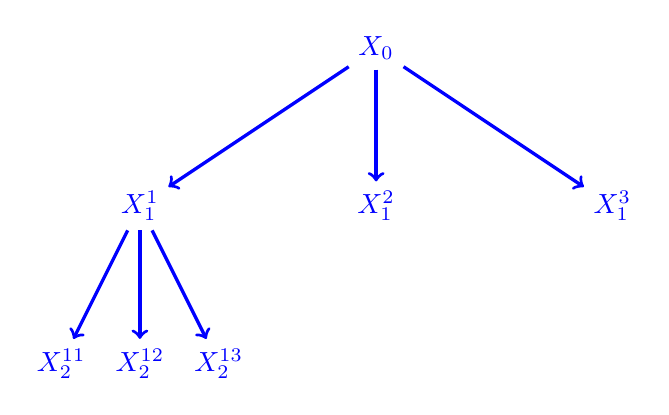
\begin{tikzpicture}
    \draw (5, 4) node[rectangle,blue] (root) {$X_0$};
    
    \foreach \branch in {1,2,3}{
        \draw (3*\branch - 1, 2) node[rectangle,blue] (1\branch) {$X_1^{\branch}$};
        \draw[->,very thick, blue] (root) -- (1\branch);
    }
    \foreach \child in {1,2,3}{
        \draw (\child + 3*1 - 3, 0) node[rectangle,blue] (21\child) {$X_2^{1\child}$};
        \draw[->,very thick,blue] (11) -- (21\child);
    }   
\end{tikzpicture} & 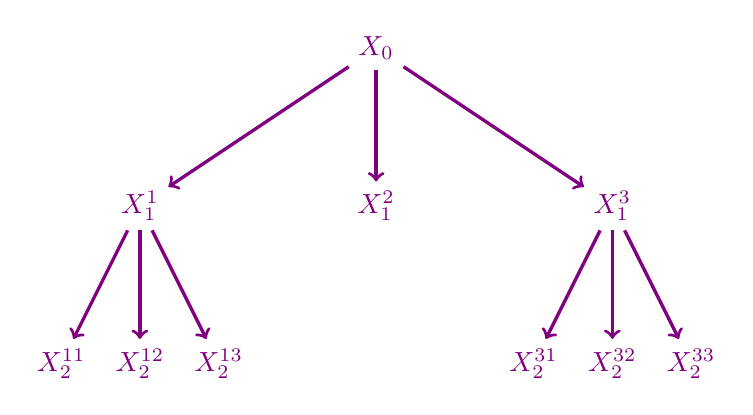
\begin{tikzpicture}
    \draw (5, 4) node[rectangle,violet] (root) {$X_0$};
    
    \foreach \branch in {1,3}{
        \draw (3*\branch - 1, 2) node[rectangle,violet] (1\branch) {$X_1^{\branch}$};
        \draw[->,very thick, violet] (root) -- (1\branch);
        \foreach \child in {1,2,3}{
            \draw (\child + 3*\branch - 3, 0) node[rectangle, violet] (2\branch\child) {$X_2^{\branch\child}$};
            \draw[->,very thick, violet] (1\branch) -- (2\branch\child);
        }
    }
    \draw (3*2 - 1, 2) node[rectangle,violet] (12) {$X_1^{2}$};
    \draw[->,very thick, violet] (root) -- (12);
\end{tikzpicture} 
\end{tabular}
\end{document}